\documentclass[t,svgnames]{beamer}
\usetheme[deutsch]{KIT}
\setbeamercovered{transparent}
\setbeamertemplate{navigation symbols}{}

\KITfoot{Worthwhile - Praxis der Softwareentwicklung WS 2011/2012}
\usepackage[utf8]{inputenc}
\usepackage{ngerman}
%\usepackage[svgnames]{xcolor}
\usepackage{listings}
\usenavigationsymbols

\lstdefinelanguage{worthwhile}
  {morekeywords={function,Boolean,Integer,_ensures,_return,return},
   morekeywords={[2]true,false},
      sensitive=true,
  morecomment=[l]{//},
  morecomment=[s]{/*}{*/},
  morestring=[b]",
}


\lstset{
   basicstyle=\ttfamily,
   keywordstyle=\bfseries\ttfamily\color{KITgreen},
   keywordstyle={[2]\bfseries\ttfamily\color{KITblue}},
   stringstyle=\color{green}\ttfamily,
   commentstyle=\color{middlegray}\ttfamily,
   emph={square}, 
   emphstyle=\color{blue}\texttt,
   emph={[2]root,base},
   emphstyle={[2]\color{yac}\texttt},
   showstringspaces=false,
   flexiblecolumns=false,
   tabsize=2,
   numbers=left,
   numberstyle=\scriptsize,
   numberblanklines=false,
   stepnumber=1,
   numbersep=10pt,
   xleftmargin=15pt,
   language=worthwhile
 }

\title{Worthwhile}
\subtitle{Abschlusspräsentation}
\author{Leon Handreke $\cdot$ Chris Hiatt $\cdot$ Stefan Orf $\cdot$ Joachim Priesner $\cdot$ Fabian Ruch $\cdot$ Matthias Wagner}

\institute[ITI]{Institut für Theoretische Informatik}

\TitleImage[trim=-24mm -35mm 0 0,width=0.9\titleimagewd]{logo.pdf}

\begin{document}

\begin{frame}
\maketitle
\end{frame}

\begin{frame}[fragile]
	\frametitle{Was machen wir?}
	
	\begin{itemize}
		\item \textbf{Programmverifikation:} Formaler Beweis, dass ein Programm seine Spezifikation erfüllt.
		\item Wichtig z.B. für sicherheitskritische Systeme
	\end{itemize}
	
		
	\begin{lstlisting}[frame=lines,mathescape=true]
		function Boolean isEven(Integer i)
		    _ensures _return = true $\Leftrightarrow $ i % 2 = 0
		{
		    if (i / 2) $ \cdot $ 2 = i {
		        return true
		    } else {
		        return false
		    }
		}
	\end{lstlisting}
	
	\begin{center}$\Rightarrow$ $$\mathtt{\forall i \in \mathbb{N} : (i / 2 \cdot 2 = i \Rightarrow i \% 2 = 0) \wedge (\neg(i / 2 \cdot 2 = i) \Rightarrow \neg(i \% 2 = 0))}$$\end{center}
	
\end{frame}

\begin{frame}
	\frametitle{Was ist Worthwhile?}
	
	\begin{columns}[c]
		\column{0.5 \textwidth}
			\begin{itemize}
			\item Mächtige Entwicklungsumgebung
			\begin{itemize}
				\item Editor
				\item Interpreter
				\item Debugger
			\end{itemize}
		\end{itemize}	
		
	\column{0.45 \textwidth}		
		
			\begin{figure}
				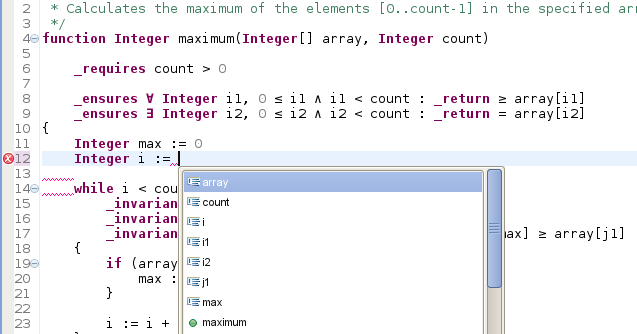
\includegraphics[width=\textwidth]{screenshot1.png}			
			\end{figure}
			
	\end{columns}	

		\setbeamercovered{invisible}	
	\pause
	
		\begin{columns}[c]
		\column{0.5 \textwidth}
			\begin{itemize}
			\item Schnittstelle für SMTLIB-kompatible Beweiser
			\begin{itemize}
				\item Transformation eines Programms in verifizierbare Formel
				\item Ausführen von Teilbeweisen (wo schlägt der Beweis fehl?)
			\end{itemize}
		\end{itemize}	
		
	\column{0.45 \textwidth}		

		\uncover<2>{\begin{figure}
				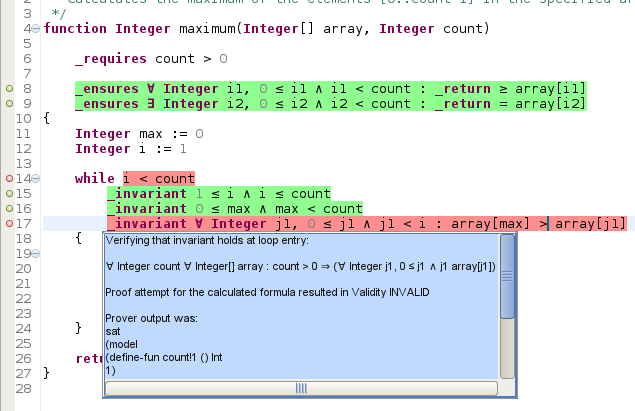
\includegraphics[width=\textwidth]{screenshot2.png}			
			\end{figure}}
	\end{columns}	
	
			\setbeamercovered{transparent}

\end{frame}

\begin{frame}
	\begin{center}
		\vfill
		\Huge{DEMO}
		\vfill		
	\end{center}
\end{frame}

\end{document}
